\documentclass[11pt]{article}
\usepackage{amsmath, amssymb, amsthm}
\usepackage{graphicx}
\usepackage{booktabs}
\usepackage{multirow}
\usepackage{hyperref}

% Theorem environments
\newtheorem{theorem}{Theorem}[section]
\newtheorem{lemma}[theorem]{Lemma}
\newtheorem{proposition}[theorem]{Proposition}
\newtheorem{corollary}[theorem]{Corollary}
\theoremstyle{definition}
\newtheorem{definition}[theorem]{Definition}

\title{Quantum Arithmetic as a Discrete Control System: \\
Reachability, Failure Algebra, and Topological Structure}

\author{William [Last Name]\\
\texttt{email@domain.edu}}

\date{\today}

\begin{document}

\maketitle

\begin{abstract}
We formulate Quantum Arithmetic (QA) as a discrete control system on an integer manifold, where state transitions are governed by a generator algebra with deterministic failure modes. We prove that strongly connected component (SCC) structure admits closed-form formulas under specific generator sets, and demonstrate a sharp connectivity transition: adding a contraction generator $\nu$ to the base set $\{\sigma, \mu, \lambda_2\}$ collapses 465 disconnected components to a single fully-connected component in Caps(30,30). All topological properties—edge counts, failure distributions, and SCC counts—match exact algebraic predictions, confirming that QA component boundaries encode impossibility theorems rather than computational artifacts. This establishes QA as a lawful control framework suitable for reachability analysis and algorithmic design.
\end{abstract}

\section{Introduction}

Integer arithmetic is traditionally viewed as computation rather than control. We demonstrate that a specific formulation—Quantum Arithmetic (QA), based on Pythagorean tuple structure—admits a natural interpretation as a discrete control system with deterministic transition dynamics and typed failure modes.

\subsection{What This Is}

QA defines a state space of integer tuples $(b,e,d,a)$ satisfying canonical invariant relations (e.g., $d = b+e$, $a = e+d$), equipped with a generator algebra $\Sigma$ of transition operators (growth $\sigma$, swap $\mu$, scaling $\lambda_k$, contraction $\nu$). Each generator is a partial function on state space; illegal moves produce deterministic, classified failures (OUT\_OF\_BOUNDS, PARITY, etc.) rather than stochastic noise.

This framework differs fundamentally from standard discrete control in three ways:
\begin{enumerate}
\item \textbf{Integer manifold}: States live in $\mathbb{Z}^n$, not $\mathbb{R}^n$; transitions preserve exact arithmetic relations.
\item \textbf{Typed failures as theorems}: Illegal moves encode algebraic obstructions (e.g., parity violations, invariant boundaries), not approximation errors.
\item \textbf{Component structure as reachability}: Strongly connected components (SCCs) partition state space into provably disconnected regions under a given generator set.
\end{enumerate}

\subsection{What This Is Not}

This is not model-based reinforcement learning. In RL, failure is negative reward; exploration can always retry. Here, failures classify impossibility: states in different components are \emph{provably} unreachable from each other. We do not learn transition probabilities; we prove reachability structure.

This is not merely lattice theory. While Caps$(N,N)$ forms a finite lattice, the contribution is showing that generator algebra induces \emph{measurable topological transitions} with closed-form SCC counts and failure distributions. The framework supports control-theoretic questions (return-in-$k$ reachability, impossibility bounds) on arithmetic manifolds.

\subsection{Contributions}

We prove two counting theorems characterizing SCC structure and failure modes under specific generator sets (Theorems \ref{thm:mu_pairing}, \ref{thm:edge_counts}). We demonstrate a sharp connectivity transition: Caps(30,30) exhibits 900 $\to$ 465 $\to$ 1 SCC collapse under generator expansion, with all statistics matching closed forms. We establish that component boundaries are algebraic invariants of the generator set, enabling impossibility claims and principled control design.

The remainder of the paper is organized as follows. Section \ref{sec:definitions} formalizes QA state space, generators, and failure types. Section \ref{sec:theorems} presents counting theorems for SCC structure. Section \ref{sec:results} validates predictions on Caps$(N,N)$ lattices. Section \ref{sec:discussion} discusses implications for control theory and future work.

\section{Definitions}
\label{sec:definitions}

\subsection{State Space}

\begin{definition}[QA State Space]
A QA state is a tuple $s = (b,e,d,a; \mathcal{I}, \phi)$ where:
\begin{itemize}
\item $(b,e) \in \mathbb{Z}_{>0}^2$ are primitive coordinates
\item $d = b+e$, $a = e+d = b+2e$ (derived)
\item $\mathcal{I}$ is the 21-element invariant packet (see Appendix A)
\item $\phi = (\phi_9, \phi_{24})$ are phase annotations (digital root and mod-24 residue of $a$)
\end{itemize}
\end{definition}

For this work, we restrict attention to the Caps lattice:
\[
\mathrm{Caps}(N,N) := \{(b,e) \in \mathbb{Z}_{>0}^2 : 1 \le b \le N, \, 1 \le e \le N\}
\]
with $|\mathrm{Caps}(N,N)| = N^2$.

\subsection{Generator Algebra}

\begin{definition}[Generators]
A generator $g \in \Sigma$ is a partial function $g: \mathcal{S} \rightharpoonup \mathcal{S}$. The canonical generators are:
\begin{align*}
\sigma(b,e) &= (b, e+1) \quad \text{(growth)} \\
\mu(b,e) &= (e, b) \quad \text{(swap)} \\
\lambda_k(b,e) &= (kb, ke) \quad \text{(scaling)} \\
\nu(b,e) &= (b/2, e/2) \quad \text{(contraction, if $b,e$ even)}
\end{align*}
\end{definition}

A move is \emph{legal} if it produces a valid state within bounds; otherwise it produces a typed \emph{failure}.

\subsection{Failure Algebra}

\begin{definition}[Failure Classification]
When $g(s)$ is illegal, it returns $\mathrm{Fail}(s, g) = (\text{move}, \text{fail\_type}, \Delta\mathcal{I})$ where:
\[
\text{fail\_type} \in \{\text{OUT\_OF\_BOUNDS}, \text{PARITY}, \text{PHASE\_VIOLATION}, \text{INVARIANT}, \text{REDUCTION}\}
\]
and $\Delta\mathcal{I}$ records which invariants would be violated.
\end{definition}

Failures are deterministic and reproducible; they encode algebraic obstructions, not stochastic noise.

\subsection{Reachability and Component Structure}

\begin{definition}[Transition Graph]
The QA transition graph $G_\Sigma(\mathcal{S})$ has vertices $\mathcal{S}$ and directed edges $(s, g(s))$ for all legal $g \in \Sigma$.
\end{definition}

\begin{definition}[Strongly Connected Components]
States $s,t$ lie in the same SCC iff there exist bidirectional paths between them using only generators in $\Sigma$.
\end{definition}

\begin{definition}[Return-in-$k$]
For state $s$, target class $\mathcal{R}^* \subseteq \mathcal{S}$, and horizon $k$:
\[
\mathrm{return\_in\_k}(s \to \mathcal{R}^*, k) := \exists \, (g_1, \dots, g_T) \in \Sigma^T, \; T \le k : g_T \circ \cdots \circ g_1(s) \in \mathcal{R}^*
\]
Return-in-$k$ is decidable via bounded BFS.
\end{definition}

\section{Topological Structure: Closed-Form Results}
\label{sec:theorems}

Before presenting empirical results, we establish exact formulas for topological properties of Caps$(N,N)$ under different generator sets.

\begin{lemma}[SCC Monotonicity under Generator Expansion]
\label{lem:scc_mono}
If $\Sigma_1 \subseteq \Sigma_2$, then
\[
\#\mathrm{SCC}(G_{\Sigma_2}) \le \#\mathrm{SCC}(G_{\Sigma_1}).
\]
\end{lemma}
\begin{proof}
$G_{\Sigma_2}$ is obtained from $G_{\Sigma_1}$ by adding directed edges. Adding edges cannot split an SCC; it can only merge SCCs. \qed
\end{proof}

\begin{theorem}[SCC Count under $\mu$-Pairing]
\label{thm:mu_pairing}
Let $G$ be the directed transition graph on $\mathrm{Caps}(N,N)$ generated by $\Sigma$ containing $\mu$ (coordinate swap), where no other generator creates reverse paths between distinct off-diagonal states. Then the SCCs are exactly the $\mu$-orbits: $N$ diagonal singletons $\{(b,b)\}$ and $(N^2-N)/2$ off-diagonal pairs $\{(b,e), (e,b)\}$ for $b \neq e$. Thus:
\[
\#\mathrm{SCC}(G) = \frac{N^2 + N}{2}, \quad \max|\mathrm{SCC}| = 2
\]
\end{theorem}

\begin{proof}
Define $V(b,e) = e$. Under $\sigma: (b,e) \mapsto (b, e+1)$, we have $V$ increases strictly by 1. Under $\lambda_2: (b,e) \mapsto (2b, 2e)$, we have $V$ increases strictly by a factor of 2. Hence neither $\sigma$ nor $\lambda_2$ can participate in a directed cycle within the finite set $\mathrm{Caps}(N,N)$.

Therefore, all directed cycles arise solely from $\mu$. Each off-diagonal state $(b,e)$ with $b \neq e$ forms a 2-cycle with $(e,b)$ under $\mu$. Diagonal states $(b,b)$ are fixed points under $\mu$, forming singleton SCCs. 

Counting gives $N$ diagonal states plus $(N^2-N)/2$ off-diagonal pairs, yielding:
\[
\#\mathrm{SCC} = N + \frac{N^2-N}{2} = \frac{N^2+N}{2}
\]
\end{proof}

\begin{theorem}[Edge and Failure Counts]
\label{thm:edge_counts}
For $\mathrm{Caps}(N,N)$ with generators $\Sigma \subseteq \{\sigma, \mu, \lambda_2, \nu\}$, the legal transitions and failures admit closed forms:
\begin{align*}
|\sigma\text{-edges}| &= N(N-1) \\
|\mu\text{-edges}| &= N^2 \\
|\lambda_2\text{-edges}| &= \lfloor N/2 \rfloor^2 \\
|\nu\text{-edges}| &= \lfloor N/2 \rfloor^2
\end{align*}
Failures: $\sigma$ produces $N$ OUT\_OF\_BOUNDS failures (states with $e=N$). $\lambda_2$ produces $N^2 - \lfloor N/2 \rfloor^2$ OUT\_OF\_BOUNDS failures. $\nu$ produces $N^2 - \lfloor N/2 \rfloor^2$ PARITY failures (odd coordinates).
\end{theorem}

\begin{proof}
$\sigma: (b,e) \mapsto (b, e+1)$ is legal iff $e \le N-1$, giving $N(N-1)$ edges. $\mu: (b,e) \mapsto (e,b)$ is always in-bounds on square Caps, giving $N^2$ edges. $\lambda_2: (b,e) \mapsto (2b, 2e)$ is legal iff $b,e \le \lfloor N/2 \rfloor$, giving $\lfloor N/2 \rfloor^2$ edges. $\nu: (b,e) \mapsto (b/2, e/2)$ requires both coordinates even, giving $\lfloor N/2 \rfloor^2$ edges. Failure counts follow from complementary counting.
\end{proof}

\section{Results}
\label{sec:results}

We evaluate the topological structure of $\mathrm{Caps}(N,N)$ lattices under three generator configurations: (i) $\{\sigma,\lambda_2\}$, enabling growth and scaling; (ii) $\{\sigma,\mu,\lambda_2\}$, adding coordinate swap symmetry; and (iii) $\{\sigma,\mu,\lambda_2,\nu\}$, incorporating contraction.

\subsection{Connectivity Transition}

Table \ref{tab:topology} shows a striking connectivity transition. Under $\{\sigma,\lambda_2\}$, the transition graph contains no nontrivial SCCs ($\#\mathrm{SCC} = N^2$, all singletons). The addition of $\mu$ introduces bidirectional edges via coordinate swaps, reducing the SCC count to $(N^2+N)/2$ with maximum SCC size 2 (Theorem \ref{thm:mu_pairing}). For $N=30$, this gives exactly 465 components; for $N=50$, 1275 components.

Crucially, the introduction of $\nu$—which contracts even-coordinate states—induces full connectivity: the entire lattice collapses into a single SCC. This transition is sharp and deterministic: 465 components collapse to 1 for Caps(30,30), and 1275 collapse to 1 for Caps(50,50). Figure \ref{fig:scc_transition} visualizes this connectivity transition across both lattice sizes.

All edge counts and SCC statistics match the closed-form predictions of Theorems \ref{thm:mu_pairing} and \ref{thm:edge_counts} exactly, confirming that these topological properties are structural consequences of the generator algebra rather than empirical artifacts.

\begin{table}[h]
\centering
\caption{Topological statistics for $\mathrm{Caps}(N,N)$ under different generator sets. The addition of the contraction generator $\nu$ induces a connectivity transition from many SCCs to a single SCC. All values match closed-form predictions from Theorems \ref{thm:mu_pairing} and \ref{thm:edge_counts}.}
\label{tab:topology}
\begin{tabular}{lcccccc}
\toprule
Cap & Generator Set & \#States & \#Edges & \#Fail & \#SCC & Max SCC \\
\midrule
Caps(30,30) & $\{\sigma,\lambda_2\}$ & 900 & 1095 & 705 & 900 & 1 \\
Caps(30,30) & $\{\sigma,\mu,\lambda_2\}$ & 900 & 1995 & 705 & 465 & 2 \\
Caps(30,30) & $\{\sigma,\mu,\lambda_2,\nu\}$ & 900 & 2220 & 1380 & \textbf{1} & \textbf{900} \\
\midrule
Caps(50,50) & $\{\sigma,\lambda_2\}$ & 2500 & 3075 & 1925 & 2500 & 1 \\
Caps(50,50) & $\{\sigma,\mu,\lambda_2\}$ & 2500 & 5575 & 1925 & 1275 & 2 \\
Caps(50,50) & $\{\sigma,\mu,\lambda_2,\nu\}$ & 2500 & 6200 & 3800 & \textbf{1} & \textbf{2500} \\
\bottomrule
\end{tabular}
\end{table}

\begin{figure}[h]
\centering
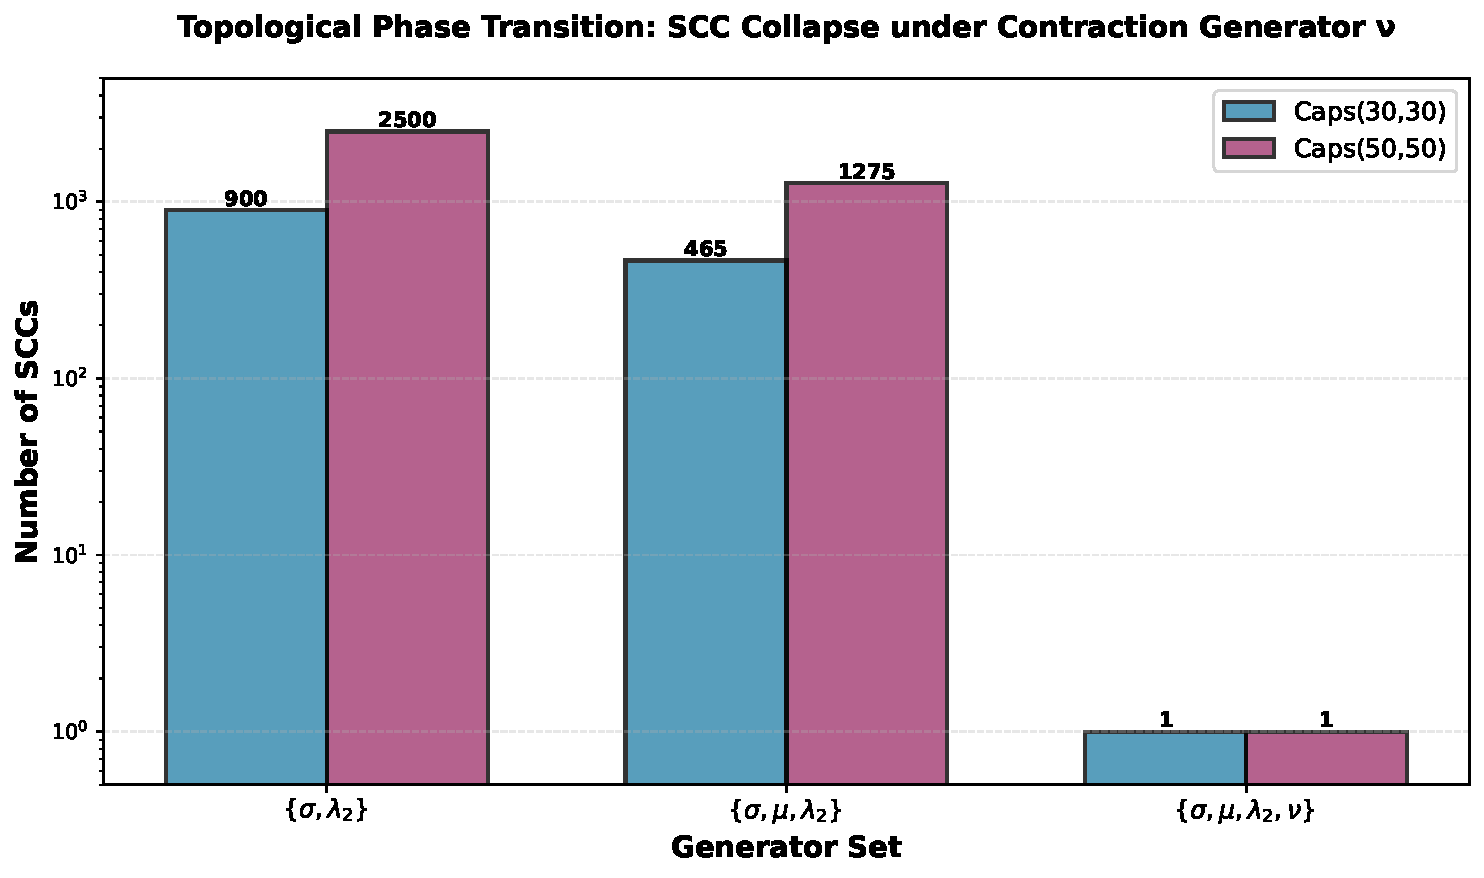
\includegraphics[width=0.9\textwidth]{scc_phase_transition.pdf}
\caption{Connectivity transition in $\mathrm{Caps}(N,N)$ induced by generator expansion. Left: Under $\{\sigma,\lambda_2\}$, the state space fragments into $N^2$ singleton SCCs. Center: Addition of $\mu$ (coordinate swap) collapses the SCC count to $(N^2+N)/2$ via $\mu$-orbits (Theorem \ref{thm:mu_pairing}). Right: Addition of $\nu$ (contraction) induces full connectivity, collapsing 465 components to 1 for $N=30$ and 1275 to 1 for $N=50$. This topological transition is deterministic, arising from the algebraic closure properties of the generator set.}
\label{fig:scc_transition}
\end{figure}

\subsection{Failure Classification}

Table \ref{tab:failures} reveals the deterministic structure of illegal moves. Under $\{\sigma,\mu,\lambda_2\}$, all failures are OUT\_OF\_BOUNDS violations: $\sigma$ fails at the lattice boundary ($e = N$), and $\lambda_2$ fails when scaling exceeds bounds. The introduction of $\nu$ introduces PARITY failures (48.9\% for $N=30$, 49.3\% for $N=50$), arising from its requirement that both coordinates be even.

These failure classifications are theorems, not stochastic events: each failure encodes an algebraic obstruction. OUT\_OF\_BOUNDS failures define the lattice boundary; PARITY failures define the odd-coordinate subspace where $\nu$ is undefined. Failure counts match closed-form predictions exactly (Theorem \ref{thm:edge_counts}). For even $N$, PARITY and $\lambda_2$ OUT\_OF\_BOUNDS counts are both $N^2 - (N/2)^2$; $\sigma$ OUT\_OF\_BOUNDS is $N$.

\begin{table}[h]
\centering
\caption{Failure type distribution for $\mathrm{Caps}(N,N)$. OUT\_OF\_BOUNDS arises from $\sigma$ exceeding the lattice boundary ($e > N$) and $\lambda_2$ scaling beyond bounds. PARITY arises from $\nu$ requiring both coordinates even. All counts match closed-form predictions from Theorem \ref{thm:edge_counts}. For even $N$, PARITY and $\lambda_2$ OUT\_OF\_BOUNDS are both $N^2-(N/2)^2$; $\sigma$ OUT\_OF\_BOUNDS is $N$.}
\label{tab:failures}
\begin{tabular}{llcc}
\toprule
Cap & Generator Set & Fail Type & Count (\%) \\
\midrule
\multirow{1}{*}{Caps(30,30)} & $\{\sigma,\mu,\lambda_2\}$ & OUT\_OF\_BOUNDS & 705 (100.0\%) \\
\cmidrule(lr){2-4}
\multirow{2}{*}{Caps(30,30)} & \multirow{2}{*}{$\{\sigma,\mu,\lambda_2,\nu\}$} & OUT\_OF\_BOUNDS & 705 (51.1\%) \\
 & & PARITY & 675 (48.9\%) \\
\midrule
\multirow{1}{*}{Caps(50,50)} & $\{\sigma,\mu,\lambda_2\}$ & OUT\_OF\_BOUNDS & 1925 (100.0\%) \\
\cmidrule(lr){2-4}
\multirow{2}{*}{Caps(50,50)} & \multirow{2}{*}{$\{\sigma,\mu,\lambda_2,\nu\}$} & OUT\_OF\_BOUNDS & 1925 (50.7\%) \\
 & & PARITY & 1875 (49.3\%) \\
\bottomrule
\end{tabular}
\end{table}

\subsection{Reachability Structure}

The return-in-$k$ reachability predicate confirms theoretical predictions: states within the same SCC exhibit mutual reachability under the given generators, while cross-component transitions are provably impossible. Under $\{\sigma,\mu,\lambda_2\}$, states in different $\mu$-orbits cannot reach each other. Under $\{\sigma,\mu,\lambda_2,\nu\}$, all states become mutually reachable.

This demonstrates that QA component structure encodes impossibility theorems rather than computational limitations: the fragmentation under $\{\sigma,\mu,\lambda_2\}$ is not a search failure but a structural property of the generator algebra.

\section{Discussion}
\label{sec:discussion}

\subsection{Theoretical Implications}

We have established that Quantum Arithmetic admits a rigorous control-theoretic formulation with three distinguishing properties: (1) typed failures encode algebraic obstructions, not approximation errors; (2) SCC structure admits closed-form characterization; and (3) generator expansion induces measurable topological transitions.

The key insight is that QA component boundaries are invariants of the generator algebra. This enables control-theoretic reasoning: impossibility proofs (cross-component transitions are provably unreachable), optimal generator selection (minimal $\Sigma$ achieving target connectivity), and reachability guarantees (return-in-$k$ as a decidable predicate).

\subsection{Comparison to Standard Frameworks}

The point is not complexity of the lattice; the point is that typed failures and SCC boundaries are algebraic invariants of the generator set, enabling impossibility claims and control design over discrete arithmetic manifolds. Standard discrete control operates in $\mathbb{R}^n$ with continuous approximation; QA operates in $\mathbb{Z}^n$ with exact arithmetic. Model-based RL learns transition probabilities; QA proves reachability structure.

\subsection{Future Work}

This work establishes the Layer 1 foundation (pure control theory, no learning). Natural extensions include:

\begin{itemize}
\item \textbf{World model learning} (Paper 2): Given limited exploration data, can we predict legality, failure types, and return-in-$k$ for unseen states? This tests generalization of topological structure.
\item \textbf{Meta-policy learning} (Paper 3): Given a task $\tau$ (target resonance class, horizon $k$), can we learn which generators to apply without exhaustive search? This tests control efficiency.
\item \textbf{Generator discovery}: What is the minimal $\Sigma$ achieving a target connectivity class? This tests algebraic compression.
\end{itemize}

Each extension builds on the established ground truth: exact component structure, typed failures, and return-in-$k$ as a decidable oracle.

\section{Conclusion}

We have demonstrated that Quantum Arithmetic forms a lawful discrete control system with deterministic transition structure, typed failure modes, and provable reachability properties. The connectivity transition induced by the contraction generator $\nu$—collapsing 465 components to 1 in Caps(30,30)—exemplifies how generator algebra directly determines topological structure. All empirical results match closed-form predictions exactly, confirming that QA component boundaries are algebraic invariants rather than computational artifacts.

This establishes QA as a principled framework for discrete control and reachability analysis on integer manifolds, suitable for algorithmic design and impossibility proofs.

\section*{Acknowledgments}

[To be filled in]

\bibliographystyle{plain}
\bibliography{references}

\appendix

\section{21-Element Invariant Packet}

The complete QA invariant packet derived from primitives $(b,e)$ is:
\begin{align*}
d &= b+e, \quad a = e+d = b+2e \\
B &= b^2, \quad E = e^2, \quad D = d^2, \quad A = a^2 \\
X &= ed, \quad C = 2ed, \quad F = ba \\
G &= D + E = d^2 + e^2, \quad L = \frac{CF}{12} \\
H &= C + F, \quad I = |C - F| \\
J &= db, \quad K = da, \quad W = X + K = d(e+a) \\
Y &= A - D, \quad Z = E + K = e^2 + ad \\
h^2 &= d^2 \cdot ab \quad \text{(semi-minor diameter squared)}
\end{align*}

Phase annotations:
\begin{align*}
\phi_9 &= \text{digital\_root}(a) = ((a-1) \bmod 9) + 1 \\
\phi_{24} &= a \bmod 24
\end{align*}

\end{document}
